\begin{figure}[ht]
\centering
\subfigure[Moduł sprężystości objętościowej]{%
    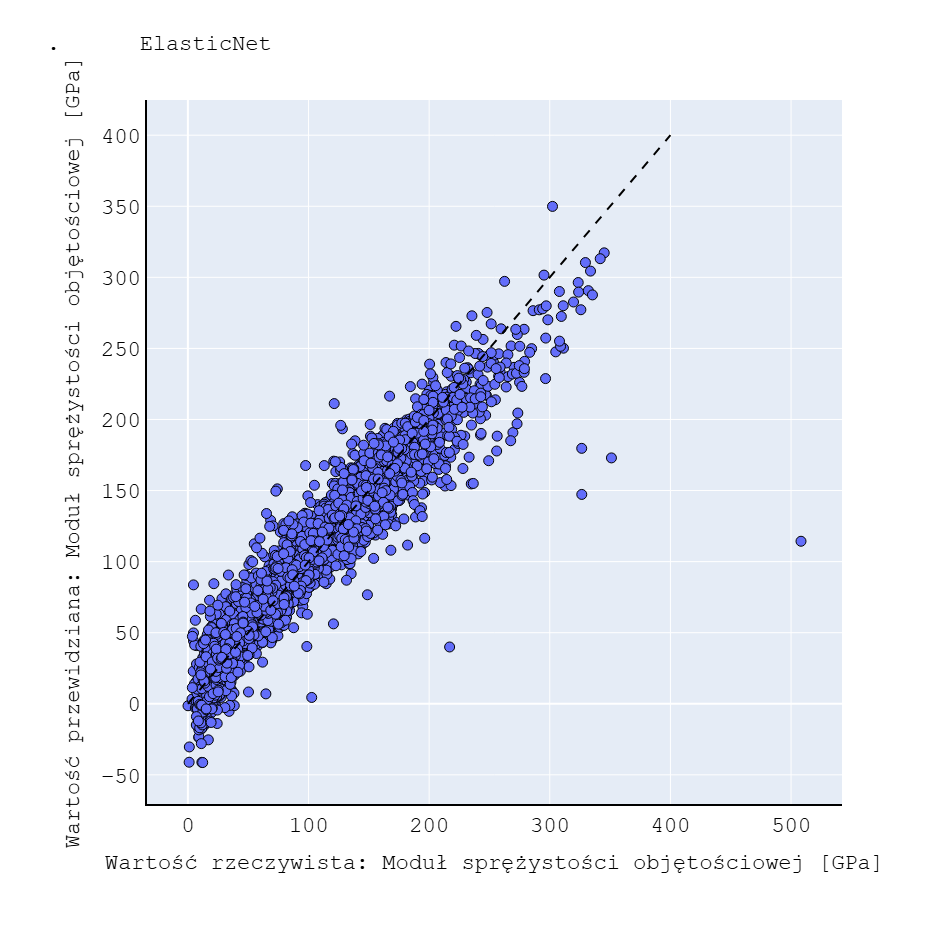
\includegraphics[width=0.48\textwidth]{images/figures/newplot (3).png}
}
\subfigure[Moduł sprężystości poprzecznej]{%
    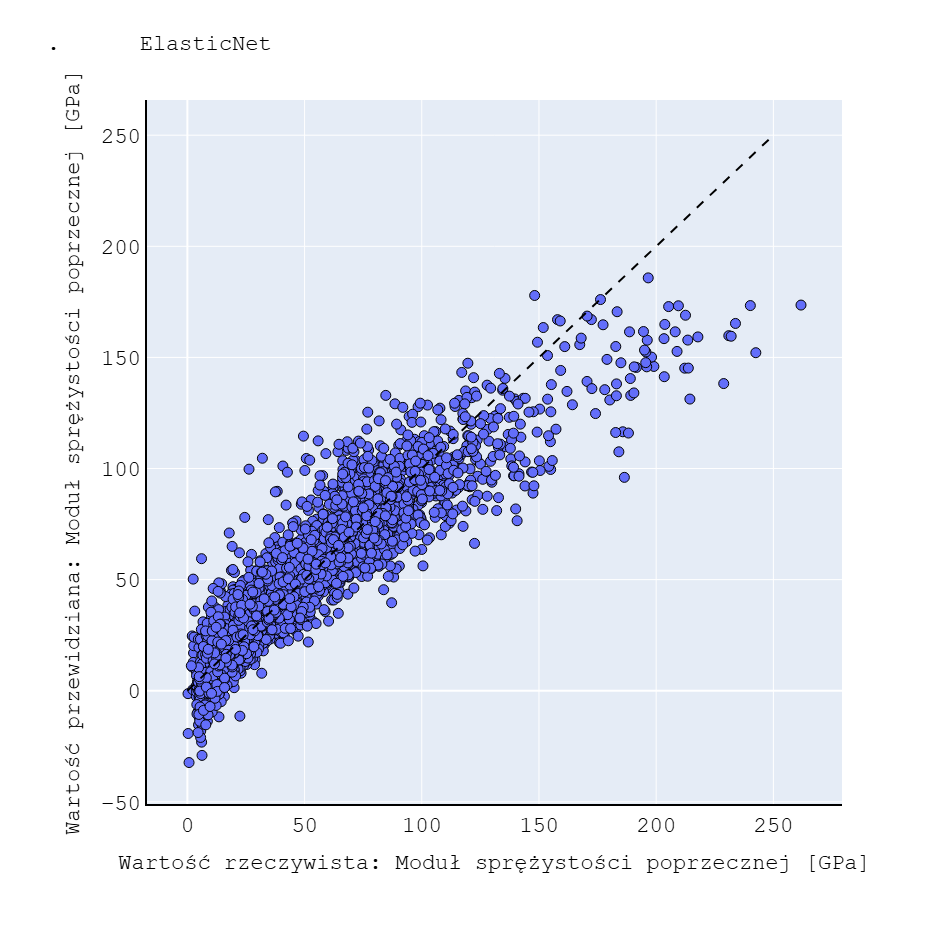
\includegraphics[width=0.48\textwidth]{images/figures/newplot (12).png}
}
\\
\subfigure[Współczynninik Anizotropii]{%
    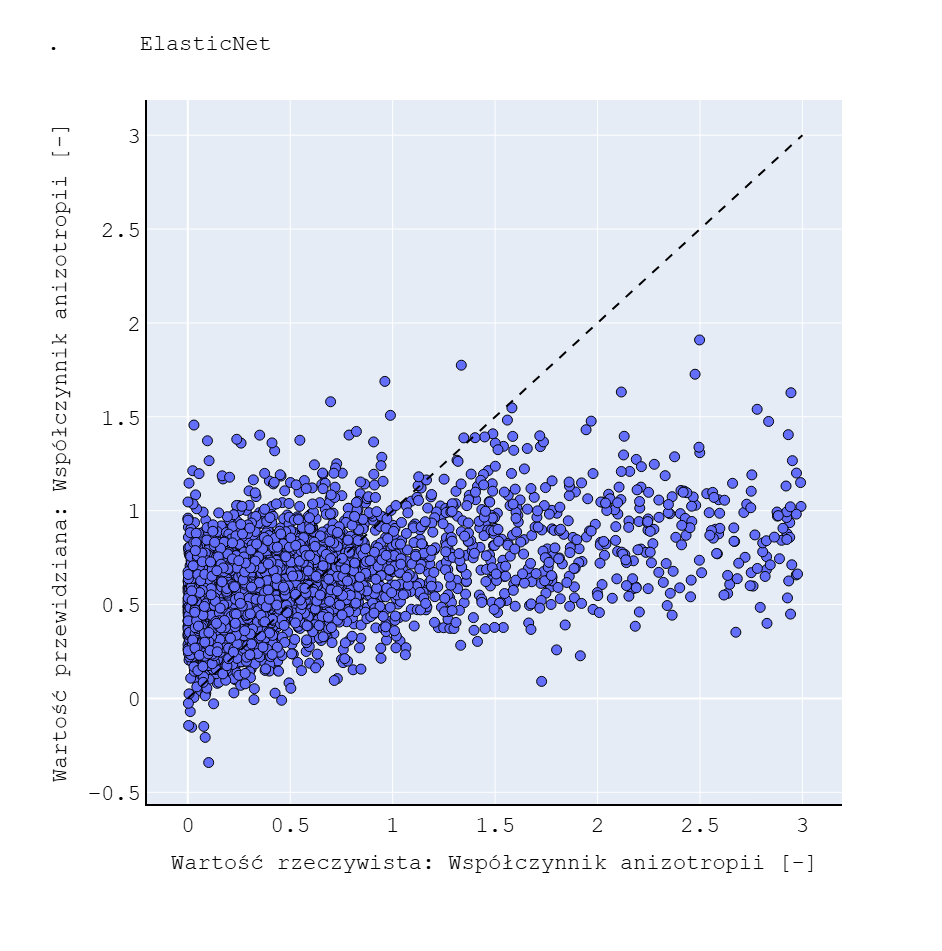
\includegraphics[width=0.48\textwidth]{images/figures/newplot (21).png}
}
\subfigure[Liczba Poisona]{%
    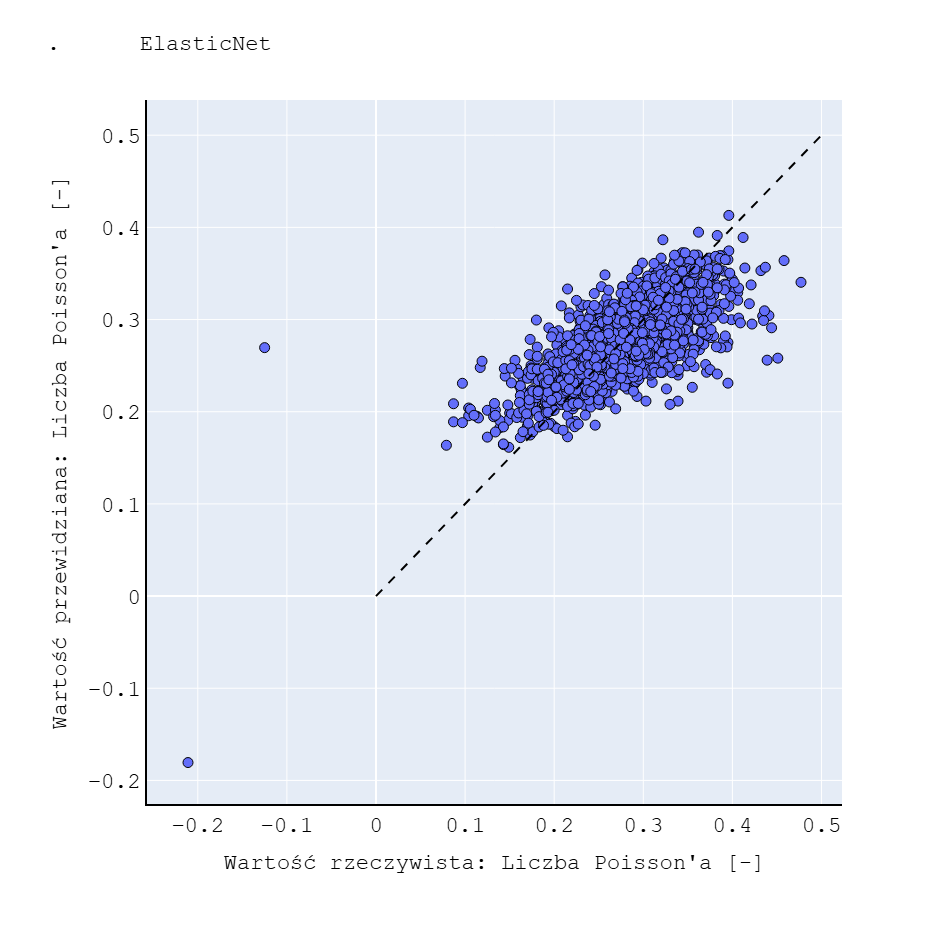
\includegraphics[width=0.48\textwidth]{images/figures/newplot (30).png}
}
\caption{Elastic Net}
\end{figure}



\clearpage